[Note: only the skeleton of this section is added, this still needs significant work]

While in the previous sections, we have investigated the various factors that could effect object memorability, an important question remembers. Now that we know what objects people remember and the factor that influence their memorability, how does the memorability of objects effect the overall image memorability? To shed light on the relationship between image memorability and object memorability, we conducted another large-scale experiment on Amazon Mechanical turk for the images in our dataset to gather their respective memorability scores. For this experiment, we followed the exact paradigm as the memory game experiment proposed in \cite{isola11}. [add details about the fillers, add details about the experiment including number of workers, number of times each image was viewed by workers and explain the consistency analysis]

After collecting the image memorability scores, we conducted several analysis to answer - if an image is highly memorable, what happens to memorability of objects inside the image (and vice versa)? For each image in the dataset, we firstly computed the maximum object memorability within the image. Figure \ref{fig:maxMem_scatter} shows the high correlation of maximum object memorability with image memorability ( $\rho = 0.43$). Although there is a high correlation between maximum object and image memorability, it still doesn't predict image memorability completely. However, table \ref{tab:imMem} also demonstrates that maximum object memorability is a very strong predictor of whether an image is highly memorable or low memorability. If we only take the topmost 20 and bottomost 20 images from the dataset, then their average max object memorability is highly correlated with the image memorability scores. Similar trend is observed for 50 most and 100 most top and bottom memorable images. This is also shown via the figure XX [show the qualitative examples here to show memorable images contain memorable objects and non-memorable images do not]. This shows although simply the max object memorability cannot predict whether an image is medium memorable, max object memorability serves as a strong features in predicting if an image is highly memorable or not. Images that are lowly memorable, is possibly due to the fact that they do not contain a single highly memorable object [refer to qual figure again]. 

\begin{table}[h]
\begin{center}
    \begin{tabular}{| l | l |}
    \hline
    Top and bottom images & max object memorability correlation \\ \hline
    20 & 0.8  \\ \hline
    50 & 0.6  \\ \hline
    100 & 0.5  \\ \hline    
    \end{tabular}
\end{center}
\caption {correlation for top and bottommost images} \label{tab:imMem}
\end{table}


\begin{figure}[t]
\centering
\subfigure{\centering 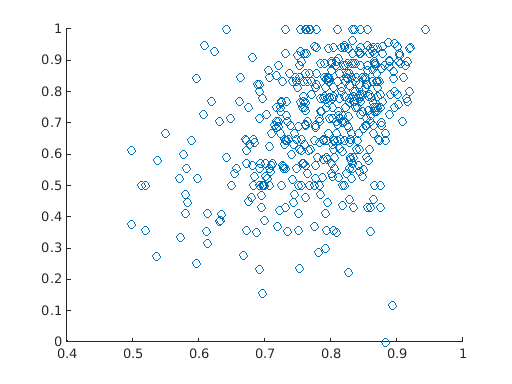
\includegraphics[width=0.4\textwidth]{figures/results/imMem/maxMem_scatter.png}}
\vspace{-5mm}\caption{\footnotesize\textbf{Correlation between max object memorability and image memorability.} add-in later. }\label{fig:maxMem_scatter}
\end{figure}